 \documentclass[technologies,article,accept,pdftex,moreauthors]{Definitions/mdpi} 
\usepackage{subcaption}
\usepackage{graphicx}% Include figure files
\usepackage{dcolumn}% Align table columns on decimal point
\usepackage{bm}% bold math

% MDPI internal commands - do not modify
\firstpage{1} 
\makeatletter 
\setcounter{page}{\@firstpage} 
\makeatother
\pubvolume{1}
\issuenum{1}
\articlenumber{0}
\pubyear{2023}
\copyrightyear{2023}
\externaleditor{Academic Editor: Pedro Antonio Gutiérrez}
\datereceived{27 September 2023} 
\daterevised{11 November 2023} % Comment out if no revised date
\dateaccepted{21 November 2023} 
\datepublished{ } 
%\datecorrected{} % For corrected papers: "Corrected: XXX" date in the original paper.
%\dateretracted{} % For corrected papers: "Retracted: XXX" date in the original paper.
\hreflink{https://doi.org/} % If needed use \linebreak

% Full title of the paper (Capitalized)
\Title{Comparing Classical and Quantum Generative Learning Models for High-Fidelity Image Synthesis}

% MDPI internal command: Title for citation in the left column
\TitleCitation{Comparing Classical and Quantum Generative Learning Models for High-Fidelity Image Synthesis} 

%\tableofcontents
% Author Orchid ID: enter ID or remove command
\newcommand{\orcidauthorA}{0000-0000-0000-000X} % Add \orcidA{} behind the author's name
%\newcommand{\orcidauthorB}{0000-0000-0000-000X} % Add \orcidB{} behind the author's name

% Authors, for the paper (add full first names)
\Author{\hl{Siddhant Jain} %MDPI: (1)Please carefully check the accuracy of names and affiliations.(2)we added affiliation numbers, please confirm
 $^{1,}$\hl %MDPI: Please confirm the corresponding author.
, \hl{Joseph Geraci} %MDPI: The name of this author is different from the one submitted online at susy.mdpi.com (Geraci Joseph). Please confirm which one is correct.
 $^{2,3,4,5}${*} and Harry \hl{E.} %MDPI: The name of this author is different from the one submitted online at susy.mdpi.com (Harry E Ruda). Please confirm which one is correct.
 Ruda $^{6}$}

%\longauthorlist{yes}

% MDPI internal command: Authors, for metadata in PDF
\AuthorNames{Siddhant Jain, Joseph Geraci and Harry E. Ruda}

% MDPI internal command: Authors, for citation in the left column
\AuthorCitation{\highlighting{Jain, S.}%MDPI: Please carefully check the accuracy of names and affiliations.
; Geraci, J.; Ruda, H.E.}
% If this is a Chicago style journal: Lastname, Firstname, Firstname Lastname, and Firstname Lastname.

% Affiliations / Addresses (Add [1] after \address if there is only one affiliation.)
\address{%
$^{1}$ \quad Division of Engineering Science, University of Toronto, \hl{Toronto, ON M5S 1A1, Canada}%MDPI: Newly added city, postcode and country information. Please confirm. same below.
\\
$^{2}$ \quad \hl{D}%MDPI: Please check the suggested address revision and order. The provided information should be arranged from subordinate to superior. same below in affiliations 3,4,5,6.
epartment of Pathology and Molecular Medicine, Queen's University, \hl{Kingston, ON K7L 3N6, Canada}; geracij@queensu.ca\\
$^{3}$ \quad \hl{Visiting Scientist} %MDPI: title/position is not allowed in address. Please revise or remove. same below in affiliations 5,6.
 for Quantum Computation and Neuroscience, University of California San Diego,  \hl{La~Jolla,~CA 92093, USA}\\
$^{4}$ \quad \hl{C}enter for Biotechnology and Genomics Medicine, Medical College of Georgia,  \hl{Augusta, GA 30912, USA}\\
$^{5}$ \quad \hl{Chief Technology Officer}, NetraMark Holdings, \hl{Toronto, ON M6P 3T1, Canada}\\
$^{6}$ \quad Stanley Meek \hl{Chair} in Nanotechnology, \hl{Centre} %MDPI: If the information provided presents more than one address, please separate the addresses into different affiliations.
 for Nanotechnology, \hl{Center} for Quantum Information and Quantum Control, Department of Electrical Engineering, University of Toronto, \hl{Toronto,~ON~M5S~1A1,~Canada}; harry.ruda@utoronto.ca}

% Contact information of the corresponding author
\corres{Correspondence: siddhant.jain@utoronto.ca} %The following comments were added in accordance with our guidelines for double-checking the accuracy and format prior to publication. Please Note: 1. We have done the initial layout for your manuscript by our layout team. Please do not change the layout. 2. Please do not delete our comments. 3. Please revise and answer all questions that we proposed. Such as: “It should be italic”; “I confirm”; “I have checked and revised all.” 4. Please directly correct on this version. 5. Please make sure that all the symbols in the paper are of the same format. 6. Please check and correct italic usage for genes, proteins and any technical terminology.
 
 

% Abstract (Do not insert blank lines, i.e., \\) 
\abstract{The field of computer vision has long grappled with the challenging task of image synthesis, which entails the creation of novel high-fidelity images. This task is underscored by the Generative Learning Trilemma, which posits that it is not possible for any image synthesis model to simultaneously excel at high-quality sampling, achieve mode convergence with diverse sample representation, and perform rapid sampling.
\highlighting{In} %MDPI: we merged paragraphs to one, please confirm
 this paper, we explore the potential of Quantum Boltzmann Machines (QBMs) for image synthesis, leveraging the D-Wave 2000Q quantum annealer. We undertake a comprehensive performance assessment of QBMs in comparison to established generative models in the field: Restricted Boltzmann Machines (RBMs), Variational Autoencoders (VAEs), Generative Adversarial Networks (GANs), and Denoising Diffusion Probabilistic Models (DDPMs). Our evaluation is grounded in widely recognized scoring metrics, including the Fréchet Inception Distance (FID), Kernel Inception Distance (KID), and Inception Scores.
\highlighting{The} results of our study indicate that QBMs do not significantly outperform the conventional models in terms of the three evaluative criteria. Moreover, QBMs have not demonstrated the capability to overcome the challenges outlined in the Trilemma of Generative Learning. Through our investigation, we contribute to the understanding of quantum computing's role in generative learning and identify critical areas for future research to enhance the capabilities of image synthesis models.}

% Keywords
\keyword{\highlighting{~~}%MDPI: Please list three to ten pertinent keywords specific to the article; yet reasonably common within the subject discipline.
}  

\begin{document} 
\section{Introduction}
\subsection{Generative Modeling}
 
Generative modelling is a class of machine learning that aims to generate novel samples from an existing dataset. Image synthesis is a subset of generative modelling applications relating to the generation of novel high-fidelity images that mimic an underlying distribution of images, known as the training set. The main types of generative models are Generative Adversarial Networks (GANs), Probabilistic models, and Variational Autoencoders (VAE), all of which are capable of high-fidelity image synthesis. In 2020, a new methodology for producing image synthesis using diffusion models was shown to produce high-quality images \cite{ho2020denoising}. In 2021, OpenAI demonstrated Denoising Diffusion Probabilistic Models' (DDPM) superiority in generating higher image sample quality than the previous state-of-the-art GANs \cite{dhariwal2021diffusion}.   %MDPI: Please consider improving the quality for displayed figures from any reference.  

Quantum annealers, namely the D-Wave 2000Q have also been shown to perform generative modelling with varied success \cite{Jain2020}\cite{Thulasidasan2016}. By taking advantage of quantum sampling and parallelization D-Wave 2000Q can hold an embedding of the latent space relating to a set of training data in an architecture of coupled qubits \cite{Amin_2018}. There are still significant research gaps relating to utilizing generative modelling on the quantum processing unit for image synthesis, especially as it relates to measuring their performance against other generative models on standard scoring methods, namely the Inception score, FID, and KID. This research aims to close this gap by investigating the efficacy of the D-Wave 2000Q quantum annealer on the problem of image synthesis.

\subsection{Trilemma of Generative Learning}
\label{trilemmaGL}
Xiao et al. describe the Trilemma of Generative Learning as the inability of any single deep generative modelling framework to solve the following requirements for wide adoption and application of image synthesis: (i) high-quality sampling, (ii) mode coverage & sample diversity, and (iii) fast and computationally inexpensive sampling \cite{xiao2022DDGAN}. Current research primarily focuses on high-quality image generation and ignores the real-world sampling constraints and the need for high diversity and mode coverage. Fast sampling allows for the generative models to be utilized in greater fast-learning applications, which require quick image synthesis, e.g. interactive image editing \cite{xiao2022DDGAN}. Diversity and mode coverage ensure generated images are not direct copies of, but are also not significantly skewed from, the training data.

\begin{figure}[H]
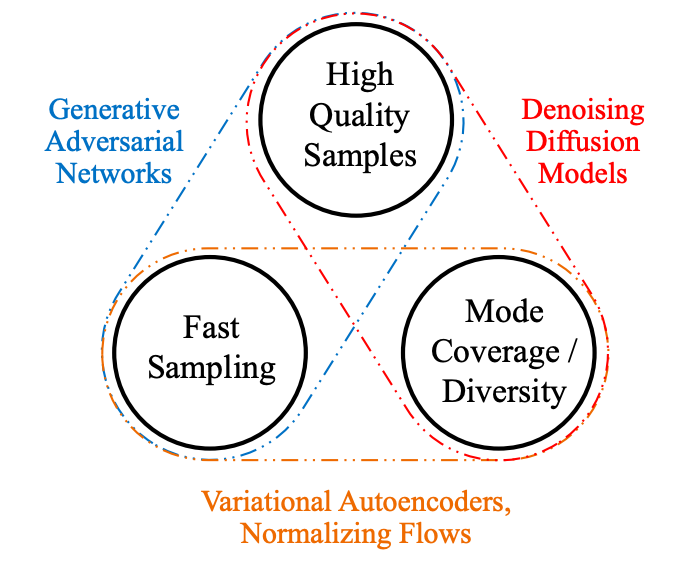
\includegraphics[width=0.9\columnwidth]{trilemma.png}% Here is how to import EPS art
\caption{\label{fig:trilemma}\hl{Generative} %MDPI: To avoid any unnecessary revision, Please cite the figure in the text and ensure the first citation of each figure appears in numerical order. 
 Learning \hl{Trilemma}%MDPI: As the copyright permission is essential for paper publication, please ensure that permission for all figures have been obtained and there is no copyright issue. If copyright is needed, please provide a citation in the following format: "Reprinted/adapted with permission from Ref. [XX]. Copyright year, copyright owner's name". More details on "Copyright and Licensing" are available via the following link: https://www.mdpi.com/ethics#10. same below. Please carefully check the information before submitting the proofread version.
~\cite{xiao2022DDGAN}. Labels show frameworks that tackle two of the three requirements well.}
\end{figure}

This paper reviews research that aims to tackle this trilemma with the D-Wave quantum annealer and attempts to determine the efficacy of modeling on the three axes of the trilemma. In doing so, the success of the quantum annealer will be tested against other classical generative modeling methodologies. Success in showing the quantum annealer's ability to produce (i) high-quality images, (ii) mode coverage and diversity, and (iii) fast sampling will demonstrate the supremacy of quantum annealers over classical methods for the balanced task of image synthesis.


\section{Background}
The trajectory of artificial intelligence in the domain of image synthesis, evolving from Restricted Boltzmann Machines (RBMs) to Denoising Diffusion Probabilistic Models (DDPMs), marks a significant technical progression. This advancement, intermediated by Variational Autoencoders (VAEs) and Generative Adversarial Networks (GANs), has driven improvements in the fidelity, diversity, and realism of generated images, while also introducing a host of model-specific challenges and computational complexities.


Before exploring generative modeling within quantum computing environments, let us provide background into classical image synthesis models, namely RBMs, VAEs, GANs, and DDPMs.


Following this, we will delve into the research of quantum annealing and its application in machine learning. The ultimate goal is to create a blueprint for image synthesis on a quantum annealer.

\subsection{Classical Image Synthesis}
\subsubsection{Restricted Boltzmann Machine}
Boltzmann Machines are a class of energy-based generative learning models. A Restricted Boltzmann Machine, a subset of Boltzmann Machines, is a fully connected bipartite graph that is segmented into visible and hidden neurons.

\vspace{-6pt}
\begin{figure}[H]
    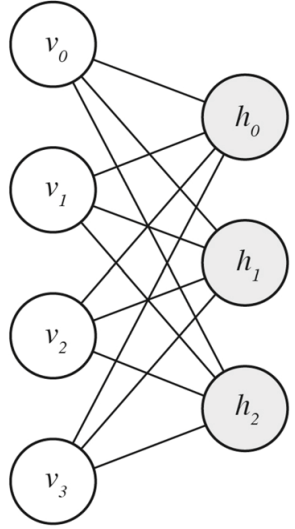
\includegraphics[width=0.53\columnwidth]{rbmgraph.png}
    \caption{\label{fig:backprop}\hl{Restricted} %MDPI: Please cite the figure in the text and ensure the first citation of each figure appears in numerical order.
 Boltzmann Machine \hl{architecture}~\cite{Jain2020}.}
\end{figure}



RBMs are generative models that embed the latent feature space in the weights between the visible and hidden layers. RBMs were first introduced in 1986 by Smolensky and were further developed by Freund and D. Haussler in 1991~\cite{Smolensky1986InformationPI,NIPS1991_33e8075e}. The energy function to minimize when training an RBM is the following~\cite{hopfield}: 
\begin{equation}
E(v, h) = -a^Tv -b^Th -v^TWh
\label{eq:rbmEnergy}
\end{equation}



Training is the process of tuning the weights matrix $W$ and bias vectors $a$ \& $b$ on the visible $v$ and hidden $h$ layers respectively. $v$ represents the visible units, i.e. the observed values; a training sample. The network assigns a probability to every possible pair of a visible and a hidden vector via this energy function \cite{Hinton2012}: 
\begin{equation}
p(v, h) = \frac{1}{Z}e^{-E(v,h)}
\end{equation}



$Z$ is the partition function given by summing over all possible pairs of $v$ and $h$~\cite{Hinton2012}. Thus, the probability of a given $v$ is: 
\begin{equation}
p(v) = \frac{1}{Z}\sum_{h} e^{-E(v,h)}
\end{equation} 
\begin{equation}
Z = \sum_{v,h}e^{-E(v,h)}
\end{equation}



The difficulty in evaluating the partition function $Z$ introduces the need to use Gibbs sampling with Contrastive Divergence Learning, introduced by Hinton et al. in 2005 \cite{CarreiraPerpin2005OnCD}. By utilizing such methods one can train the RBM quickly via gradient descent, similar to other neural networks. By adding more hidden layers a deeper embedding can be captured by the model; such a system is called a Deep Belief Network (DBN).


RBMs, while of little note in the modern landscape of machine learning research due to their limited performance and relatively slow training times, are of particular note to this research as they have direct parallels with both the architecture of the D-Wave 2000Q quantum processor and the method by which they reduce the total energy of their respective systems. RBMs also have limited applications in computer vision but were an important advancement in the field of generative modelling as a whole.



\subsubsection{Variational Autoencoder}
A Variational Autoencoder (VAE) is a generative machine learning model developed in 2013 composed of a neural network that is able to generate novel high-fidelity images, texts, sounds, etc. \cite{kingma2014autoencoding}.


Autoencoders seek to compress an input space into a compressed latent representation from which the original input space can be recovered~\cite{kingma2014autoencoding}. Variational Autoencoders improve upon traditional Autoencoders by recognizing the input space has an underlying distribution and seeks to learn the parameters of that distribution~\cite{kingma2014autoencoding}. Once trained, VAEs can be used to generate novel data, similar to the input space, by removing the encoding layers and exploring the latent space~\cite{kingma2014autoencoding}. Exploring the latent space is simply treating the latent compression layer as an input layer and observing the output of the VAE for various inputs. VAEs marked the first reliable way to generate somewhat high-fidelity images using machine learning \cite{rocca_2021}.

\begin{figure}[H]
    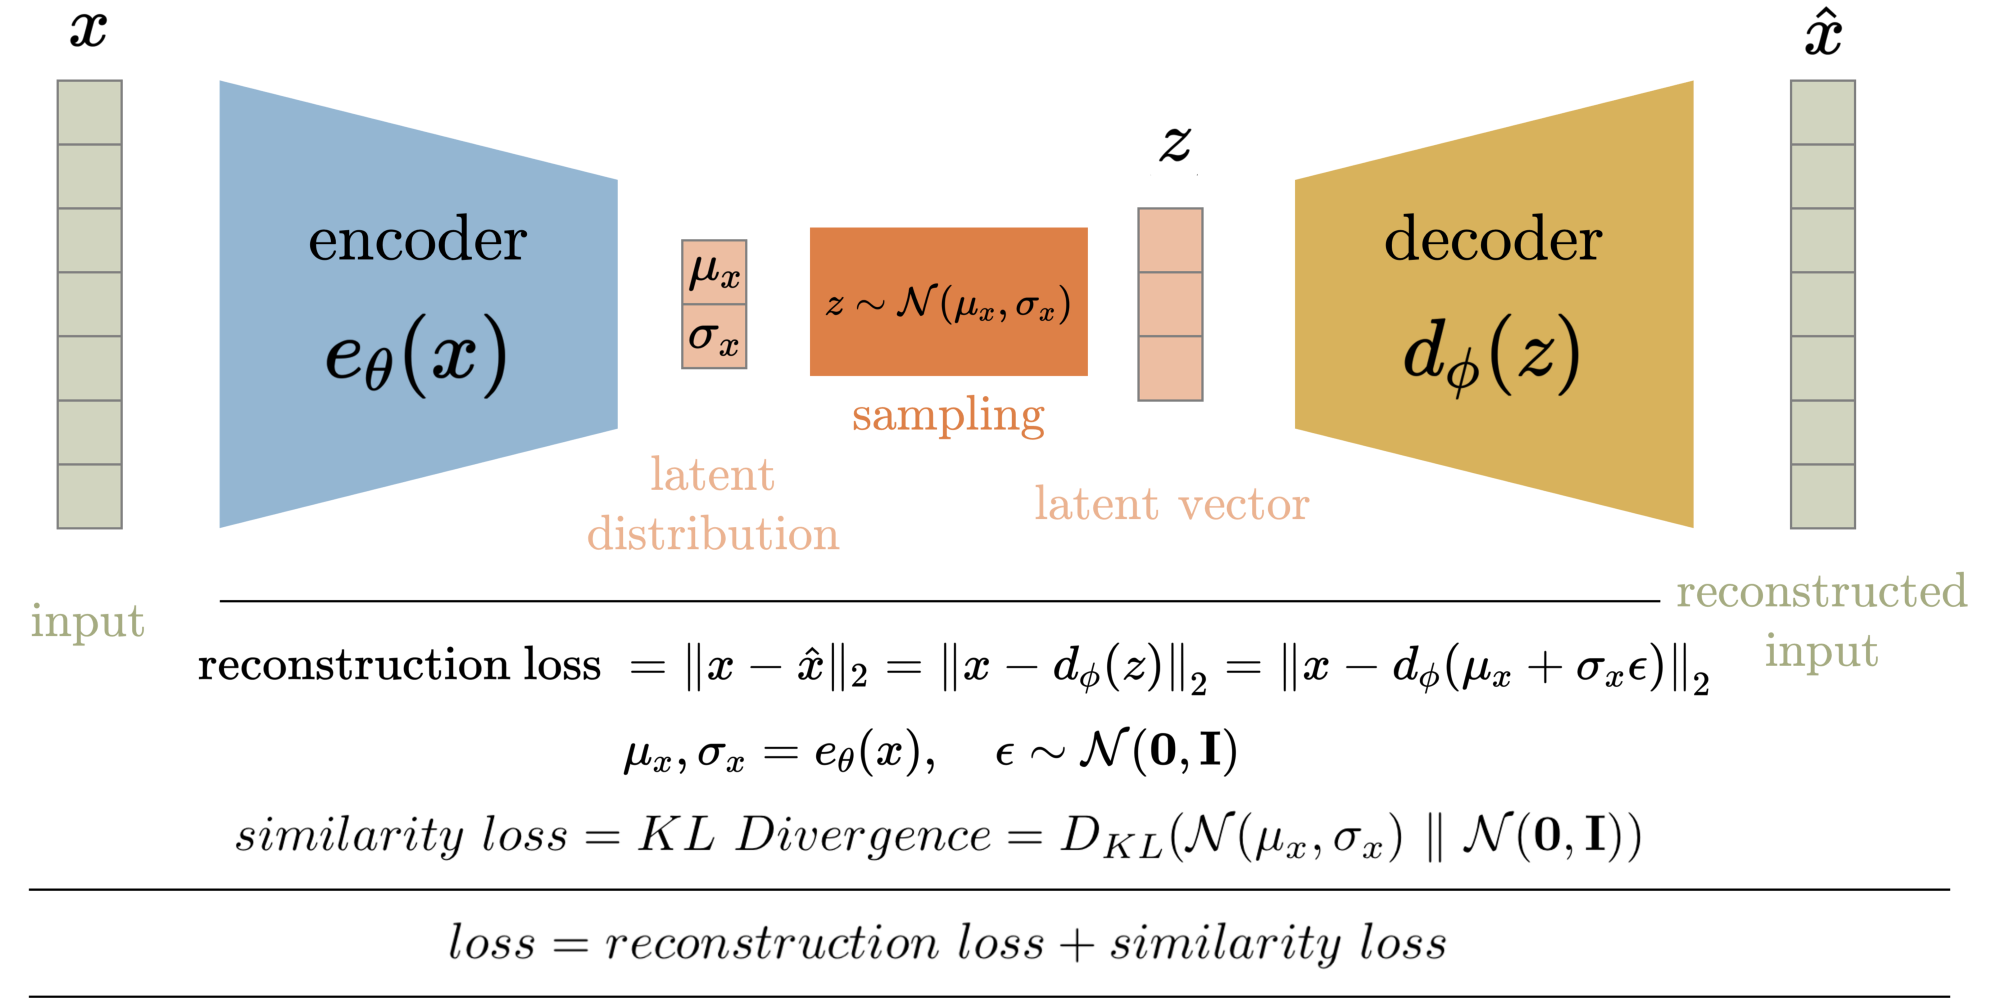
\includegraphics[width=.99\columnwidth]{vae.png}
    \caption{\label{fig:vae}\hl{Variational} %MDPI: (1)Please cite the figure in the text and ensure the first citation of each figure appears in numerical order. (2)figures 3,5 label id are same, please revise
 Autoencoder \hl{architecture}~\cite{rocca_2021}.}
\end{figure}

\subsubsection{Generative Adversarial Networks}
\label{VG}
The most significant development in high-fidelity generative image synthesis was in 2014 with the introduction of  GANs by Ian Goodfellow et al.~\cite{goodfellow2014generative}. Goodfellow et al. propose a two-player minimax game composed of a generator model (G) and a discriminator model (D). As the game progresses, both the generator and discriminator models improve.


GANs are trained via an adversarial contest between the generator model (G) and discriminator model (D)~\cite{goodfellow2014generative}. $x$ contains samples from both the training set and $p_g$, the images generated by G. $D(x;\theta_d)$ outputs the probability that $x$ originates from the training dataset as opposed to $p_g$. Meanwhile, $G(z, \theta_g)$ outputs $p_g$ given noise $z$. G's goal is to fool D while D aims to reliably differentiate real training data from data generated by G. The loss function for G is $log(1 - D(G(z)))$. Thus, the value/loss function, error, of a GAN is represented as:
\begin{equation}
% \begin{split}
\mathrm{\underset{G}{min} \:\underset{D}{max} } \;V (D, G) = E_{x\sim p_{data}(x)} [log D(x)] \\
+ E_{z\sim p_{z}(z)} [log(1 - D(G(z)))]
% \end{split}
\end{equation}  
\vspace{-12pt}

\begin{figure}[H]
    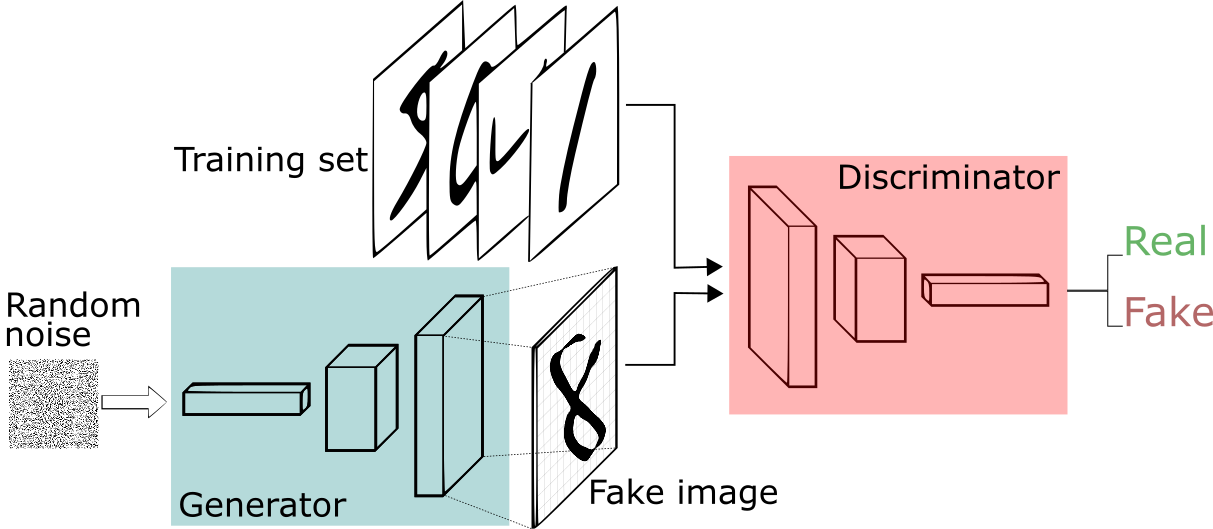
\includegraphics[width=\columnwidth]{GANs.png}
    \caption{\hl{GANs} %MDPI: Please cite the figure in the text and ensure the first citation of each figure appears in numerical order. 
 \hl{architecture}~\cite{Yan2021}.\label{fig:GAN}}
\end{figure}



Both G and D are trained simultaneously. This algorithm allows for lock-step improvements to both G and D. Towards the conclusion of training, G becomes a powerful image generator, which closely replicates the input space, i.e., training data.


GANs have several shortcomings that make them difficult to train. Due to the adversarial nature of GAN training the model can face the issue of Vanishing Gradients, when the discriminator develops more quickly than the generator consequently correctly predicting every $x$ and leaving no error to train on for the generator \cite{google}. Another common issue is Mode Collapse when the generator learns to generate a particularly successful $x$ such that the discriminator is consistently fooled and the generator continues to only produce that singular $x$ and has no variability in image generation \cite{google}. Both Vanishing Gradients and Mode Collapse are consequences of one of the adversarial models improving faster than the other.


\subsubsection{Denoising Diffusion Probabilistic Model}

DDPMs are a recent development proposed by Jonathan Ho et al. (2020) inspired by nonequilibrium thermodynamics that produces high-fidelity image synthesis using a parameterized Markov chain \cite{ho2020denoising}. Beginning with the training sample, each step of the Markov chain adds a single layer of Gaussian noise. A neural network is trained on parameterizing these additional Gaussian noise layers to reverse the process from random noise to a high-fidelity image.

\begin{figure}[H]
    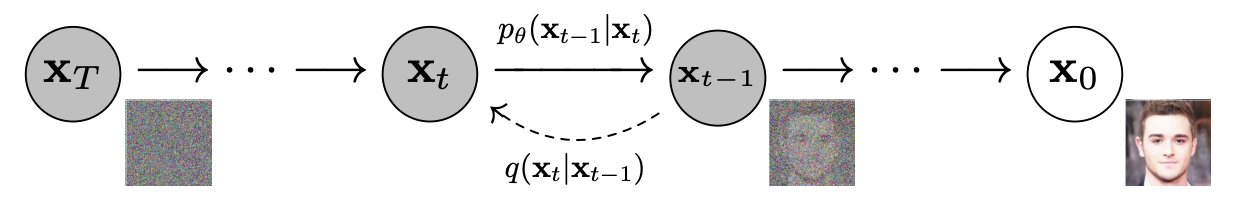
\includegraphics[width=\columnwidth]{ddpm.png}
    \caption{\label{fig:vae}\hl{DDPM} %MDPI:  %MDPI: (1)Please cite the figure in the text and ensure the first citation of each figure appears in numerical order. (2)figures 3,5 label id are same, please revise
 Markov \hl{chain}~\cite{ho2020denoising}.}
\end{figure}


$q_\theta(x_t|x_{t-1} )$  represents the forward process, adding Gaussian noise, and $p_\theta(x_{t-1}|x_t )$ represents the reverse process, denoising. The reverse process is captured by training.

\begin{equation}
p_\theta(x_0) :=\int p_\theta(x_{0:T} ) dx_{1:T}
\end{equation}
where

\begin{equation}
p_\theta(x_{0:T}) := p(x_T)\prod_{t=1}^{T} p_\theta(x_{t-1}|x)
\end{equation}
and

\begin{equation}
p_\theta(x_{t-1}|x) := \mathcal{N}(x_{t-1};\mu_\theta(x_t,t); \Sigma_\theta(x_t,t))
\end{equation}

For clarity, we remind the reader that $\mathcal{N}(x_{t-1};\mu_\theta(x_t,t); \Sigma_\theta(x_t,t))$ is the normal distribution with mean $\mu_\theta(x_t,t)$ and covariance matrix $\Sigma_\theta(x_t,t)$. The loss function for a DDPM is as \hl{follows:} %MDPI: Please confirm if the bold in following equation should be retained. And the rest of whole paper is same.
\begin{equation}
L := \mathbf{E}_q[-\mathrm{log} p(x_T) - \sum_{t\ge1}\mathrm{log} \frac{p_\theta(x_{t-1}|x )}{q_\theta(x|x_{t-1} )}]
\end{equation}


\textls[-9]{Using a U-Net and a CNN with upsampling, with stochastic gradient descent and $T~=~1000$}, Ho et al. were able to generate samples with an impressive, but not state-of-the-art, FID score of 0.317 on the CIFAR10 dataset. On CelebA-HQ 256~$\times$~256, the team generated the novel images in Figure~\ref{fig:DDPMCeleb}.

\begin{figure}[H]
    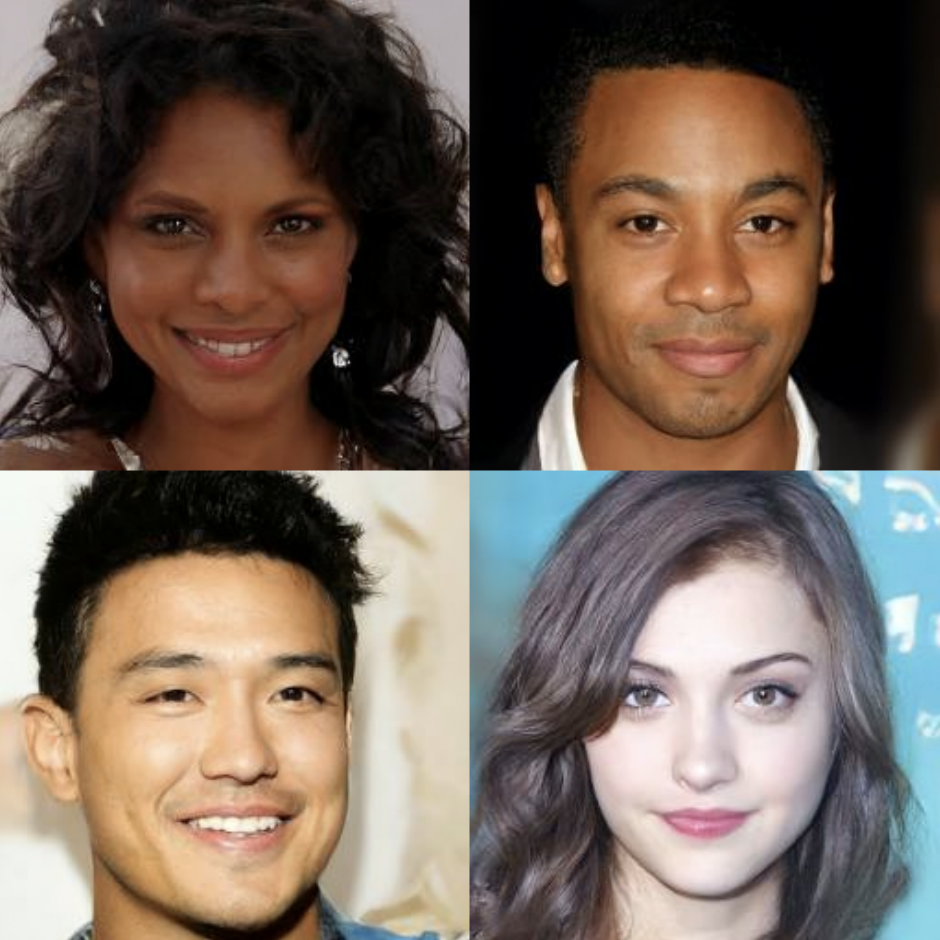
\includegraphics[width=.95\columnwidth]{celeb.png}
    \caption{\label{fig:DDPMCeleb}\hl{Generated} %MDPI: Please cite the figure in the text and ensure the first citation of each figure appears in numerical order.
 samples on CelebA-HQ 256~$\times$~256 by \hl{DDPM}~\cite{ho2020denoising}.}
\end{figure}



In 2021, Dhariwal et al. at OpenAI made improvements upon the original DDPM parameters, and it achieved state-of-the-art FID scores of 2.97 on ImageNet 128~$\times$~128, 4.59 on ImageNet 256~$\times$~256, and 7.72 on ImageNet 512~$\times$~512~\cite{dhariwal2021diffusion}.

The first improvement is not to set $\Sigma_\theta(x_t, t) $ as a constant but rather as the following:
\begin{equation}
\Sigma_\theta(x_t, t) = \mathrm{exp}(v \mathrm{log} \beta_t + (1 - v) \mathrm{log} \tilde{\beta_t})
\end{equation}
where $\beta_t$ and  $\tilde{\beta_t}$ correspond to the upper and lower bounds of the Gaussian variance.


Dhariwal et al. also explore the following architectural changes; note: attention heads refer to embedding blocks in the U-Net~\cite{dhariwal2021diffusion}:
\begin{itemize}
\item Increasing depth versus width, holding model size relatively constant.
\item Increasing the number of attention heads.
\item Using attention at 32~$\times$~32, 16~$\times$~16, and 8~$\times$~8 resolutions rather than only at 16~$\times$~16.
\item Using the BigGAN residual block for upsampling and downsampling the activations.
\item Rescaling residual connections with $\frac{1}{\sqrt{2}}$.
\end{itemize}


With these changes, Dhariwal et al. were able to demonstrate their DDPM beating GANs in every single class by FID score and establishing DDPMs as the new state-of-the-art for image synthesis~\cite{dhariwal2021diffusion}.

\subsection{Quantum Machine Learning}
\subsubsection{Quantum Boltzmann Machine}
Energy-based machine learning models, such as the RBM, seek to minimize an energy function. Recall:

\begin{equation}
p(v) = \frac{\sum_{h} e^{-E(v,h)}}{\sum_{v,h}e^{-E(v,h)}}
\end{equation}
is maximized when $E(v,h)$ is minimized.

\begin{equation}
E(v, h) = -a^Tv -b^Th -v^TWh
\end{equation}
or, in its expanded form
\begin{equation}
E(v, h) = - \sum_{i} v_i \cdot a_i - \sum_{j} h_j \cdot b_j - \sum_{i} \sum_{j} v_i \cdot W_{ij} \cdot h_j
\end{equation}

Recall also that this energy function is intractable for all $v$ and $h$, thus RBMs are trained via Contrastive Divergence~\cite{trainingrbms}.

The D-Wave 2000Q via the Ising model is able to minimize an energy function via coupled qubits, taking advantage of entanglement. The energy function for the Ising model is the following {Hamiltonian}: 
\begin{equation}
E_{\text{ising}}(\mathbf{s}) = \sum_{i=1}^N h_i s_i + \sum_{i=1}^N \sum_{j=i+1}^N J_{i,j} s_i s_j
\end{equation}



The $s_i \in \{-1, +1\}$ represents the qubit spin state, with spin up and spin down effectively. $h_i$ is the bias term provided by the external magnetic field, and $J_{i,j}$ captures the coefficients for the coupling between qubits~\cite{dwavedocs}. Solving for the ground state of an Ising model is NP-hard, but by taking advantage of the QPU's ability to better simulate quantum systems, we can solve this problem more efficiently~\cite{monte}.


Clamping neurons is the process of affixing certain qubits to specific values, namely the data being trained on. By clamping the neurons $v$ and $h$ onto the qubits, applying an external magnetic field equivalent to the biasing parameters $a$ and $b$, and setting the coupling parameters to match those of $W$ (and to 0 for absent or intralayer edges), the RBM can be effectively translated into a format suitable for a quantum annealer. The resulting model is known as a Quantum Boltzmann Machine (QBM) and is similarly trained using QPU-specific Gibbs sampling methods~\cite{dwavedocs,qpugibbs}.



Increased sampling from the quantum annealer leads to a more comprehensive representation of the Hamiltonian's energy landscape. The process of training a QBM involves adjusting the couplings based on this acquired information. The D-Wave 2000Q has the qubit coupling architecture in Figure~\ref{fig:chimera}.

\subsubsection{Image Classification}
The field of Quantum Machine Learning (QML) applied to computer vision is still quite nascent. Most QML research focuses on classification tasks, particularly using quantum support vector machines, decision trees, nearest neighbors, annealing-based classifiers, and variation classifiers~\cite{classifiers}.  Wei et al. propose a Quantum Convolutional Neural Network with capabilities for spatial filtering, image smoothing, sharpening, and edge detection, along with MNIST digit recognition, with a lower computation complexity than classical counterparts~\cite{quantumCNN}. Such research provides a valuable precursor to the exploration of QML for image synthesis.

\begin{figure}[H]
    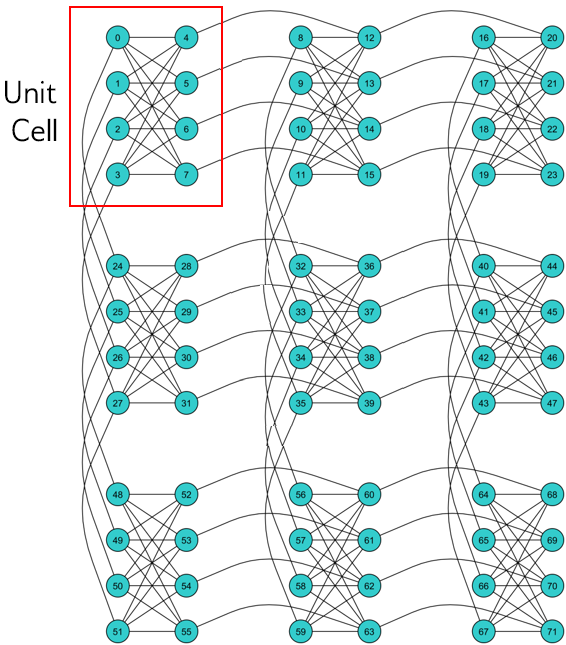
\includegraphics[width=0.95\columnwidth]{chimera.png}
    \caption{\label{fig:chimera}D-Wave Quantum Processing Unit (QPU) topology Chimera \hl{graph}~\cite{dwavedocs}.}
\end{figure}



\subsubsection{Image Synthesis}
In 2020, Sleeman et al. demonstrated the D-Wave QUBO's ability to generate images mimicking the MNIST hand-drawn digits and Fashion MNIST datasets~\cite{qmlimggen}. Due to the limited number of qubits available, Sleeman et al. create an encoding of the images via a convolutional autoencoder, feed the encoding to a QBM, and finally reverse the process to perform image synthesis. The model architecture is provided in Figure~\ref{fig:hybridML}.

\begin{figure}[H]
    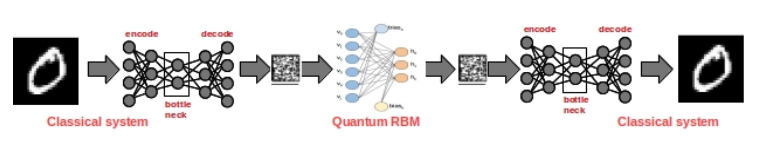
\includegraphics[width=\textwidth]{qmlimgimg.png}
    \caption{\label{fig:hybridML}\hl{Hybrid} %MDPI: The contents of this figure are not legible. Please replace the image with one of a sufficiently high resolution (min. 1000 pixels width/height, or a resolution of 300 dpi or higher).
 Approach that used a Classical Autoencoder to map the image space to a compressed space~\cite{qmlimggen}.}
\end{figure}


In their research, Sleeman et al. contrast the performance of their QBM with that of a traditional RBM, in addition to assessing the efficacy of the autoencoder's encoding capabilities. Despite showcasing the potential of the D-Wave 2000Q in aiding image synthesis, the authors do not juxtapose their findings with those of other classical generative modeling methods. Furthermore, the omission of FID, KID, and Inception scores for their proposed models restricts the breadth of comparison between the QBM and its classical counterparts.

\section{Methods}
\subsection{Goal}
To reiterate, the goal of this research is to train the D-Wave 2000Q quantum annealer on image synthesis (generative image creation) and compare the results both quantitatively and qualitatively against existing classical models. Secondly, the goal is to determine the quantum annealer's efficacy at cracking the challenges outlined in Section \ref{trilemmaGL}, specifically the Trilemma of Generative Learning. 



Additionally, our research aims to close many of the gaps in Sleeman et al.'s study. Namely:

\begin{itemize}
    \item perform the image synthesis directly on the QBM,
    \item evaluate the performance of the QBM against a(n) RBM, VAE, GAN, and DDPM,
    \item evaluate various generative modeling methods on FID, KID, and Inception scores,
    \item model a richer image dataset, CIFAR-10.
\end{itemize}

\subsection{Data}
We utilize a standardized dataset, CIFAR-10, for all of our experiments. The CIFAR-10 dataset consists of sixty thousand 32 by 32 three-channel (color) images in ten uniform classes~\cite{CIFAR}. The data were initially collected in 2009 by Alex Krizhevsky, Vinod Nair, and Geoffrey Hinton and have become the standard for machine learning research relating to computer vision~\cite{Krizhevsky09learningmultiple}. One of the primary reasons CIFAR-10 is so popular is because the small image sizes allow for quick training and testing of new models~\cite{ai_progress_measurement}. In addition, the ubiquity of testing models on CIFAR-10 allows researchers to quickly benchmark their model performance against prior research~\cite{ai_progress_measurement}.


\begin{figure}[H]
    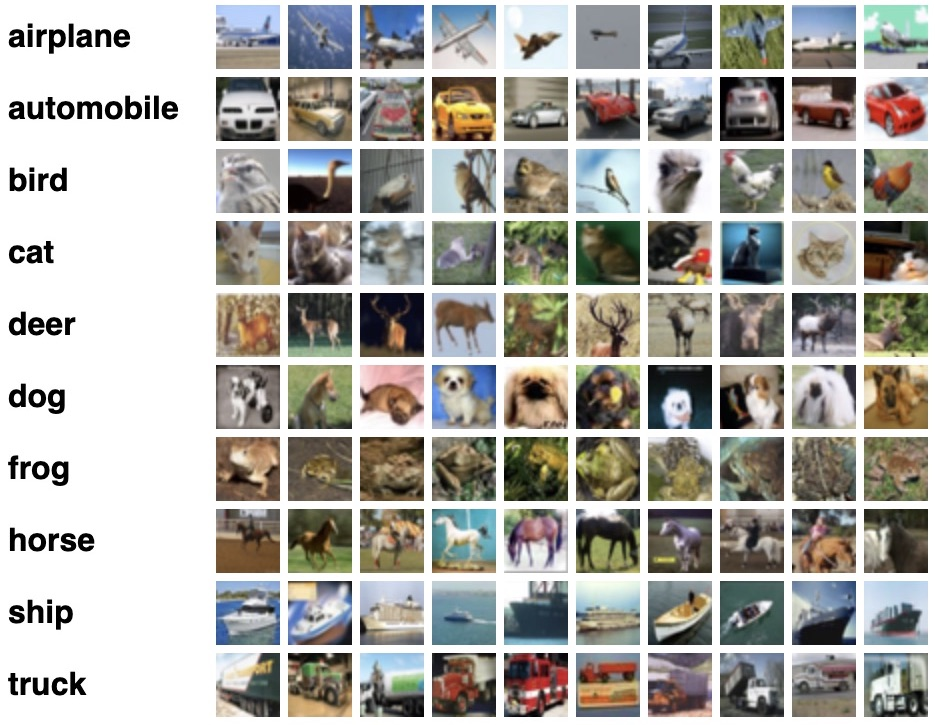
\includegraphics[width=.9\columnwidth]{cifar10.jpeg}
    \caption{\label{fig:cifar10}\hl{Ten} %MDPI: Please cite the figure in the text and ensure the first citation of each figure appears in numerical order.
 random images from each class of CIFAR-10 with respective class \hl{labels}~\cite{CIFAR}.}
\end{figure}


The images in CIFAR-10 are exclusive to photographs of discrete distinct objects on a generally neutral background. The dataset contains photographs, which are two-dimensional projections of three-dimensional objects, from various angles.


\subsection{Classical Models}

To establish a benchmark and facilitate the comparison of results between novel quantum machine learning methods and existing generative image synthesis techniques, we initially trained and tested a series of classical models on the CIFAR-10 dataset. The classical models we trained on were the following: (i) RBM, (ii) VAE, (iii) GANs, and (iv) DDPM. Initially, we adopted a uniform approach, training each model with the same learning rate, batch size, and number of epochs to standardize results. However, this method led to significant challenges due to the varying rates of convergence among the models, causing an imbalance in result quality and impeding our analysis. Consequently, we adjusted our approach to individually optimize the hyperparameters for each model within the bounds of available time and resources. This adjustment yielded higher-quality results, offering a more equitable comparison across models. We concluded the training of each model when additional epochs resulted in insignificant improvements in model loss, a term left intentionally vague to accommodate training variability across models. An exception to this approach was made for the DDPM, which demanded considerable computational power, prompting us to conclude the experiment after 30,000 iterations.


\subsection{Quantum Model}
\label{binarize}
For the quantum model, the training images were also normalized by mean and variance, identically to the preprocessing for the classical models. Since quantum bits can only be clamped to binary values and not floating point numbers, the data also had to be binarized. This process involves converting each input vector into 100 vectors where the representation of 1s in each row reflects the floating point number between 0--1, as pictured in Figure~\ref{fig: binarize}.

\begin{figure}[H]
    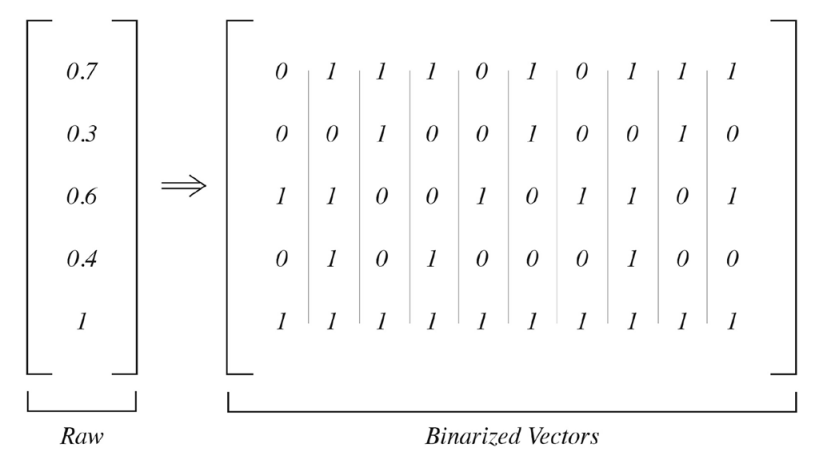
\includegraphics[width=0.99\columnwidth]{binarize.png}
    \caption{\label{fig: binarize} Binarization of a normalized vector to a set of binary vectors~\cite{Jain2020}.}
\end{figure}


The D-Wave 2000Q quantum annealer is trained by mapping the architecture of an RBM onto the QPU Chimera graph, thus creating a QBM~\cite{dwavedocs}. The visible, i.e., input, nodes are clamped with the training data, and the hidden layer is sampled from. As we increase sampling, we gain a better understanding of the energy landscape and can better update the weights (i.e., inter-qubit coupling coefficients)~\cite{Jain2020}.


Due to limitations with the number of available qubits on the D-Wave 2000Q being 2048, and user resource allocation challenges, our experiments are limited. To resolve this constraint, each image was split into four distinct squares along the $x$ and $y$ axes. Thus, each training image was 16 $\times$ 16 $\times$ 3 for an input vector size of 768.

\subsection{Hyper-Parameters} 
The hyper-parameters were determined by conducting grid search hyper-tuning. Since DDPMs are trained via an iterative process, unbatched, they require significantly more epochs, as reflected in Table~\ref{tab:hyperparams}.

\begin{table}[H]
\caption{\label{tab:hyperparams}Final hyper-parameters used for respective model training.}
\tabcolsep=.5cm
\begin{tabular}{cccccc}
\toprule
& \textbf{QBM} & \textbf{RBM} & \textbf{VAE} & \textbf{GAN} & \textbf{DDPM}\\
\midrule
 Epochs & 10 & 10 & 50 & 50 & 30,000\\ 
 Batch Size & 256 & 256 & 512 & 128 & - \\ 
\hl{\#} %MDPI: Please check if the # need be explained.
 of Hidden Nodes & 128 & 2500 & 32 & 64 & 32 \\ 
 Learning Rate ($10^{-3}$) & 0.0035 & 0.0035 & 0.2 & 0.2 & 0.2\\
\bottomrule
\end{tabular}
\end{table}


\subsection{Metrics}
\label{metrics_}
\subsubsection{Inception Score}
Inception score measures two primary attributes of the generated images: (i) the fidelity of the images, i.e., the image distinctly belongs to a particular class and (ii) the diversity of the generated images~\cite{mack_2019}. The Inception classifier is a Convolutional Neural Network (CNN) built by Google and trained on the ImageNet dataset consisting of 14~million images and 1000 classes~\cite{inception_model}.


(i) Fidelity is captured by the probability distribution produced as classification output by the Inception classifier on a generated image~\cite{mack_2019}. Note that a highly skewed distribution with a single peak indicates that the Inception classifier is able to identify the image as belonging to a specific class with high confidence. Therefore, the image is considered high fidelity.



(ii) Diversity is captured by summing all the probability distributions produced for individually generated classes. The uniform nature of the resultant sum of distributions is indicative of the diversity of the generated images. E.g., a model trained on CIFAR-10 that only manages to produce high-fidelity images of dogs would severely fail to be diverse.



The average of the K-L Divergences between the produced probability distribution and the summed distribution is the final Inception score, capturing both diversity and fidelity.
Rigorously, each generated image $x_i$ is classified using the Inception classifier to obtain the probability distribution $p(y|x_i)$ over classes $y$~\cite{isscore}. The marginal distributions are provided by: 

\begin{equation}
p(y) = \frac{1}{N} \sum_{i=1}^{N} p(y|x_i)
\end{equation}

From which the K-L Divergence may be computed by the \hl{following}%MDPI: Reference citation is not allowed in equation, so we moved here. Please confirm this revision. same below.
~\cite{isscore}:
\begin{equation}
    D_{\text{KL}}(p(y|x_i) || p(y)) = \sum_{y} p(y|x_i) \log \left( \frac{p(y|x_i)}{p(y)} \right)
\end{equation}

\textls[-25]{Take the expected value of these K-L Divergences over all $N$ generated \hl{images}~\cite{isscore}:} 
\begin{equation}
    \mathbb{E}_{x}[D_{\text{KL}}(p(y|x) || p(y))] = \frac{1}{N} \sum_{i=1}^{N} D_{\text{KL}}(p(y|x_i) || p(y)) 
\end{equation}

Finally, we exponentiate the value above to evaluate an Inception \hl{score}~\cite{isscore}:
\begin{equation}
\text{IS}(G) = \exp (E_{x\sim pg} \mathcal{D}_{KL}(p(y|x) || p(y))
\end{equation}

\subsubsection{Fréchet Inception Distance (FID)}
Fréchet Inception Distance improves upon the Inception score by capturing the relationship between the generated images against the training images, whereas the Inception score only captures the characteristics of the generated images against each other and their classifications. The Inception classifier, used to determine the Inception score, also embeds a feature vector. I.e., the architecture of the Inception classifier captures the salient features of the images it is trained on.



The FID score is determined by taking the Wasserstein metric between the two multivariate Gaussian distributions of the feature vectors for the training and generated images on the Inception model~\cite{NIPS2017_8a1d6947}. Simply, the dissimilarity between the features found in the training and generated data. This is an improvement upon the Inception score since it captures the higher-level features that would be more human-identifiable when comparing model performance. The Gaussian distributions of the feature vector for the generated images and the training images are $N(\mu, \Sigma)$ and $N(\mu_w, \Sigma_w)$, respectively~\cite{fid_gan}. The Wasserstein metric, resulting in the FID score, is as \hl{follows}~\cite{fid_gan}:
\begin{equation}
\text{FID}=||\mu -\mu _{w}||_{2}^{2}+\operatorname {tr} (\Sigma +\Sigma _{w}-2(\Sigma ^{1/2}\Sigma _{w}\Sigma ^{1/2})^{1/2})
\end{equation}


\subsubsection{Kernel Inception Distance (KID)}
KID measures the maximum mean discrepancy of the distributions of training and generated images by randomly sampling from them both~\cite{MMD_KID}. KID does not specifically account for differences in high-level features and rather compares the raw distributions more directly.


Specifically, for generator $X$ with probability measure $\mathbb{P}$ and random variable $Y$ with probability measure $\mathbb{Q}$, we \hl{have}~\cite{MMD_KID}:
\begin{equation}
\mathcal{D}_F(\mathbb{P},\mathbb{Q}) = \sup_{f\in F}\mathbb{E}_\mathbb{P}f(X) - \mathbb{E}_\mathbb{Q}f(Y) 
\end{equation}

\subsubsection{Quantitative Metrics}
The following table summarizes the three quantitative metrics used to evaluate model performance:

\begin{table}[H]
\caption{\hl{Summary} %MDPI: Please cite the table in the text and ensure that the first citation of each table appears in numerical order.
 of quantitative metrics for generative image synthesis evaluation.\label{tab:metrics}} 
\tabcolsep=.3cm 
    \begin{tabular}{cp{8cm}c} 
\toprule
  \textbf{Metric}& \textbf{Description} &\textbf{Performance}\\ 
 \midrule        
 {{Inception}} & K-L Divergence between conditional and marginal label distributions over generated data & Higher is better\\   \midrule   
 FID & Wasserstein distance between multivariate Gaussians fitted to data embedded into a feature space & Lower is better\\   \midrule   
 KID & Measures the dissimilarity between two probability distributions $P_r$ and $P_g$ using samples drawn independently from each distribution & Lower is better\\
 \bottomrule
    \end{tabular} 
\end{table}


\subsubsection{Qualitative Metrics}
Our qualitative evaluation was performed by analyzing the visual discernment of generated images in relation to their respective classes less stringently. This approach aims to foster a broader discussion about the applicability of such models and their effectiveness.

\section{Results}
\subsection{Restricted Boltzmann Machine (RBM)}

The generated images by the RBM include a high degree of brightly-colored noise. Interestingly this noise is concentrated in sections of the image with high texture, i.e., high variance of pixel values. Notice the image of the cat in the bottom-center on Figure~\ref{fig:rbmresults}b has a great deal of noise at the edges of and inside the boundaries of the cat itself, but not in the blank white space surrounding it. This demonstrates a high degree of internode interference in the hidden layer. That is, areas with large pixel variance influence the surrounding pixels greatly and often cause bright spots to appear as a result.


\subsection{Variational Autoencoder (VAE)}
The generated images from the VAE are incredibly high fidelity. Notably, the VAE results liken superresolution. Notice the decrease in image blur/noise from the input images. Since the VAE encodes an embedding of the training data, some features, such as the exact color of the vehicle in the top left corner in Figure~\ref{fig:vaeresults}b, are lost, but the outline of the vehicle and the background are sharpened. This demonstrates the VAE is capturing features exceptionally well.

\subsection{Generative Adversarial Networks (GANs)}

The GAN is able to produce some images with high fidelity, namely the cat in the top left corner and the dog in the bottom right corner of Figure~\ref{fig:ganresults}b, but struggles with the sharpness of the images. Humans looking at the majority of the images produced could easily determine they are computer generated. In addition, the GAN was uniquely difficult to train, requiring retraining dozens of times in order to avoid Vanishing Gradients and Mode Collapse. Recall from \hl{Section} %MDPI: Newly added. Please confirm. same below.
 \ref{VG}, Vanishing Gradients and Mode Collapse are issues that arise from the discriminator or generator improving significantly faster than the counterpart and dominating future training, thus failing to improve both models adequately and defeating the adversarial training nature of the network.

\subsection{Denoising Diffusion Probabilistic Model (DDPM)}
\label{ddpm_result_}
The quality of the results for the DDPM are limited by the computational power available to run the experiment. DDPMs are state-of-the-art for image generation when scored on fidelity but require several hours of training on a Tensor Processing Unit (TPU). A TPU can perform one to two orders of magnitude more operations than an equivalent GPU per second~\cite{googlecloud}. Without access to these Google-exclusive TPUs, we were unable to replicate state-of-the-art generation results.  

\subsection{Quantum Boltzmann Machine (QBM)}
\label{qbm_result_}
Recall the QBM required training images to be split and restitched into four independent squares for training due to qubit limitations. This splitting and restitching has a distinct influence on the resultant generated images. Notice the generated images have distinct features in each quadrant of the image. These features are often from various classes and appear stitched together because they are. Notice how the image in the bottom row, second from the rightmost column has features of a car, a house, and a concrete background.

\begin{figure}[H] 
        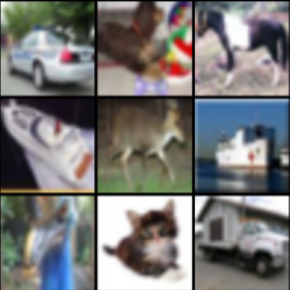
\includegraphics[width=.77\linewidth]{rbmin.png}\\
\text{~~~~~~~~~~~~~~~~~~~~~~~~~~~~~~~~~~~~~~~~~~~~~~~~~~~~~~~~}(\textbf{a}) 
        \label{fig:rbmin} \\
        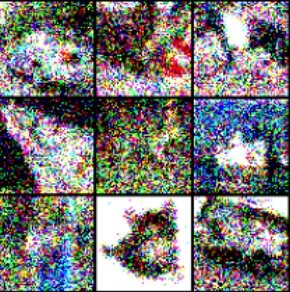
\includegraphics[width=.77\linewidth]{rbmout.png}\\
 \text{~~~~~~~~~~~~~~~~~~~~~~~~~~~~~~~~~~~~~~~~~~~~~~~~~~~~~~~~}(\textbf{b}) 
        \label{fig:rbmout} 
    \caption{RBM-generated image synthesis output from respective input. \hl{(\textbf{a}) RBM input images; (\textbf{b})~RBM output images.}%MDPI: We moved the subfigure explanations into the figure caption. Please confirm. same below.
\label{fig:rbmresults}} 
\end{figure}

\vspace{-9pt}




\begin{figure}[H]
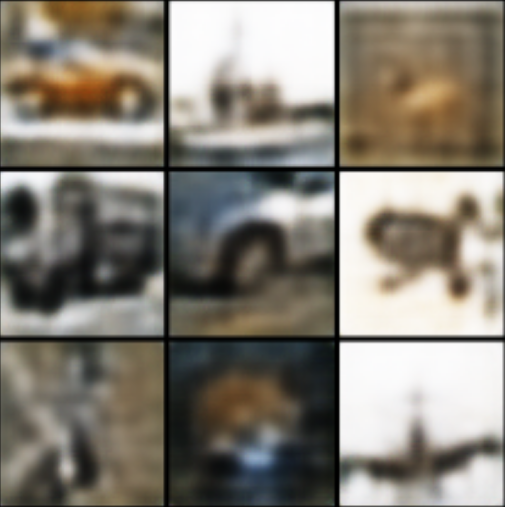
\includegraphics[width=.77\linewidth]{vaein.png}\\
\text{~~~~~~~~~~~~~~~~~~~~~~~~~~~~~~~~~~~~~~~~~~~~~~~~~~~~~~~~}(\textbf{a}) 
        \label{fig:vaein} \\
        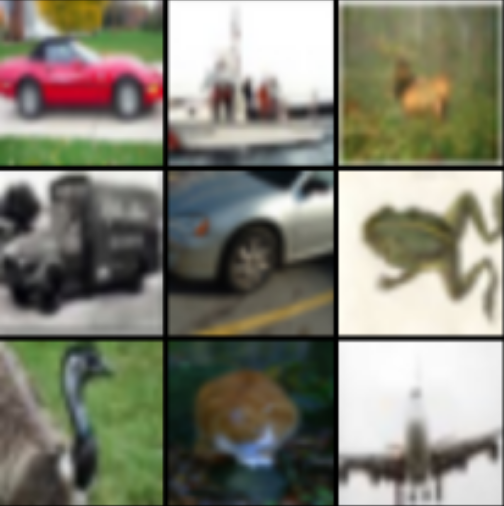
\includegraphics[width=.77\linewidth]{vaeout.png}\\
\text{~~~~~~~~~~~~~~~~~~~~~~~~~~~~~~~~~~~~~~~~~~~~~~~~~~~~~~~~}(\textbf{b}) 
        \label{fig:vaeout}  
    \caption{VAE-generated image synthesis output from respective input. \hl{(\textbf{a}) VAE input images; (\textbf{b})~VAE output images.}\label{fig:vaeresults}} 
\end{figure} 
\vspace{-9pt}

\begin{figure}[H]
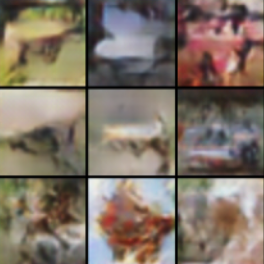
\includegraphics[width=.77\linewidth]{ganin.png}\\
\text{~~~~~~~~~~~~~~~~~~~~~~~~~~~~~~~~~~~~~~~~~~~~~~~~~~~~~~~~}(\textbf{a}) 
        \label{fig:ganin} \\
        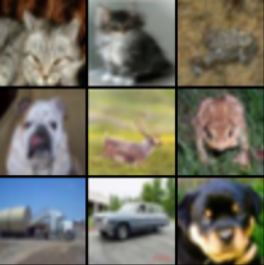
\includegraphics[width=.77\linewidth]{ganout.png}\\
\text{~~~~~~~~~~~~~~~~~~~~~~~~~~~~~~~~~~~~~~~~~~~~~~~~~~~~~~~~}(\textbf{b}) 
        \label{fig:ganout} 
    \caption{GAN-generated image synthesis output from respective input. \hl{(\textbf{a}) GAN input images; (\textbf{b})~GAN output images.}}
    \label{fig:ganresults}
\end{figure}





\vspace{-9pt}

\begin{figure}[H]
    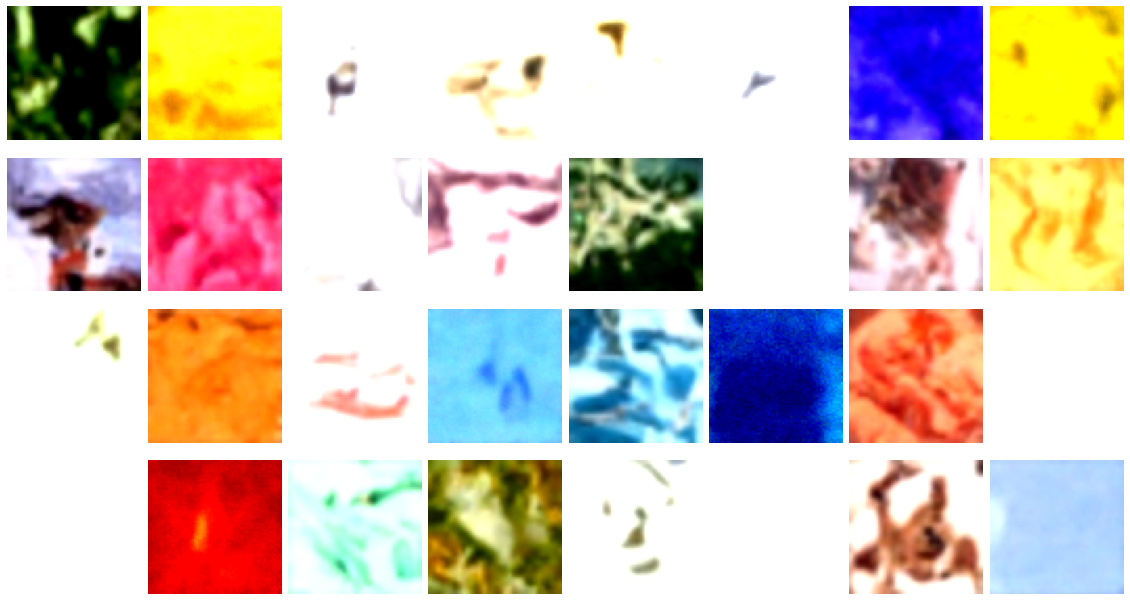
\includegraphics[width=.98\columnwidth]{ddpmout.png}
    \caption{\label{fig:ddpmresults}\hl{DDPM-generated} %MDPI: Please cite the figure in the text and ensure the first citation of each figure appears in numerical order.
image synthesis output from random noise inputs.}
\end{figure}
 


\section{Analysis}
\subsection{Scores} 
The following analyses reference the results captured in Table~\ref{tab: results}.

\begin{table}[H]
\caption{Quantitative results of generative modeling on Inception score, FID, and KID metrics.\label{tab: results}} 
%\tabcolsep=.62cm
\begin{tabularx}{\textwidth}{CCCCCC}
\toprule
& \textbf{QBM} & \textbf{RBM} & \textbf{VAE} & \textbf{GAN} & \textbf{DDPM}\\
\midrule
 Inception& 1.77 &3.84& 7.87& 2.72 & 3.319\\ 
 FID& 210.83&379.65 & 93.48 & 122.49 & 307.51\\ 
 KID&0.068&0.191 & 0.024 & 0.033 & 0.586 \\ 
 \bottomrule
\end{tabularx} 
\end{table}





\subsubsection{Inception Score}
On Inception scores, the QBM performed significantly worse than the classical models. This means that the diversity and fidelity of the QBM-generated images were significantly worse than those produced via existing classical methods. The VAE produced an exceptionally high Inception score, suggesting the images were both distinctly single-class labelled and the results produced an equal variety of results across classes. Qualitative observation of the produced samples is consistent with this score, as the produced images are of high fidelity and varied classes. Note that Figure~\ref{fig:vaeresults}b has distinct images of vehicles, animals, planes, etc.


Interestingly the DDPM produced a middling Inception score despite producing images that were of exceptionally low fidelity. This is because the Inception score measures the K-L Divergence between the single sample classification probability distribution and the summed distribution. While the image fidelity may be low, the overall summed distribution is fairly uniform due to the high variance of results, resulting in a higher K-L Divergence than naively expected.

\subsubsection{Fréchet Inception Distance}
The QBM produced the median FID score on the generated images, performing better than the RBM and DDPM but worse than the GAN and VAE. Recall the primary difference between the FID score and other metrics is the model's ability to extract and replicate salient features of the training data. The VAE and GAN do this exceptionally well, producing images that have distinct features that are easily observable. Notice \mbox{Figures~\ref{fig:vaeresults}b and \ref{fig:ganresults}b} both contain images that have easily identifiable features, namely the animals and vehicles in each set of generated images. Despite these images mimicking the input image very closely, especially for Figure~\ref{fig:vaeresults}, the FID score only captures the distance between the features present in produced vs. training images, not the diversity of the images themselves.


Alternatively, the images produced by the DDPM and RBM have a distinct lack of identifiable features. To the human eye, Figure~\ref{fig:rbmresults}b does reflect the general lines and edges of the input found in Figure~\ref{fig:rbmresults}a, yet the Inception classifier fails to capture these features in its embedding, likely due to the high levels of surrounding noise with bright values. Note that brightly colored pixels are caused by large RGB (red-green-blue) values, which will have a larger effect upon the convolutional filters, which rely on matrix multiplication. This can have an undue negative effect on feature extraction and thus lead to lower FID scores. DDPMs face issues relating to a general lack of distinctive features produced. As discussed in \hl{Section} \ref{ddpm_result_}, the computational limitations did not allow for adequate training and can thus account for the lack of effective feature generation.


As discussed in \hl{Section} \ref{qbm_result_}, the stitching and restitching of images cause features from multiple classes to be present in a single image, despite each feature being of moderately high fidelity.  This restitching has negative consequences on the FID score and, given more qubits, could be improved upon but clamping entire images to the QPU directly.


\subsubsection{Kernel Inception Distance}
As with the FID score, the QBM produced the median score on the generated images yet skewed lower and thus achieved better results than the DDPM and GAN. The DDPM once again suffers from a lack of computing power and thus performs significantly worse than other models. The VAE and RBM performed exceptionally well, indicating the models' superior ability to generate samples that are distributed similarly to the training set.


KID is the metric on which the QBM performed comparatively best. This means that while the QBM lacks the ability to represent features in its generated images well and struggles to produce diverse, high-fidelity images, it can capture the underlying distribution of training images with its generated images moderately well. This result is significant because the fidelity of generated images should improve with increases in the number of qubits and better error correction, but a promising KID score is indicative that the QBM is adequately capturing the essence of image generation. Qualitatively, from Figure~\ref{fig:qbmresults}, it is clear the QBM can capture some meaningful image features from the training set but struggles with fidelity, i.e., distinct objects, clear boundaries, textured backgrounds, etc.

\begin{figure}[H]
    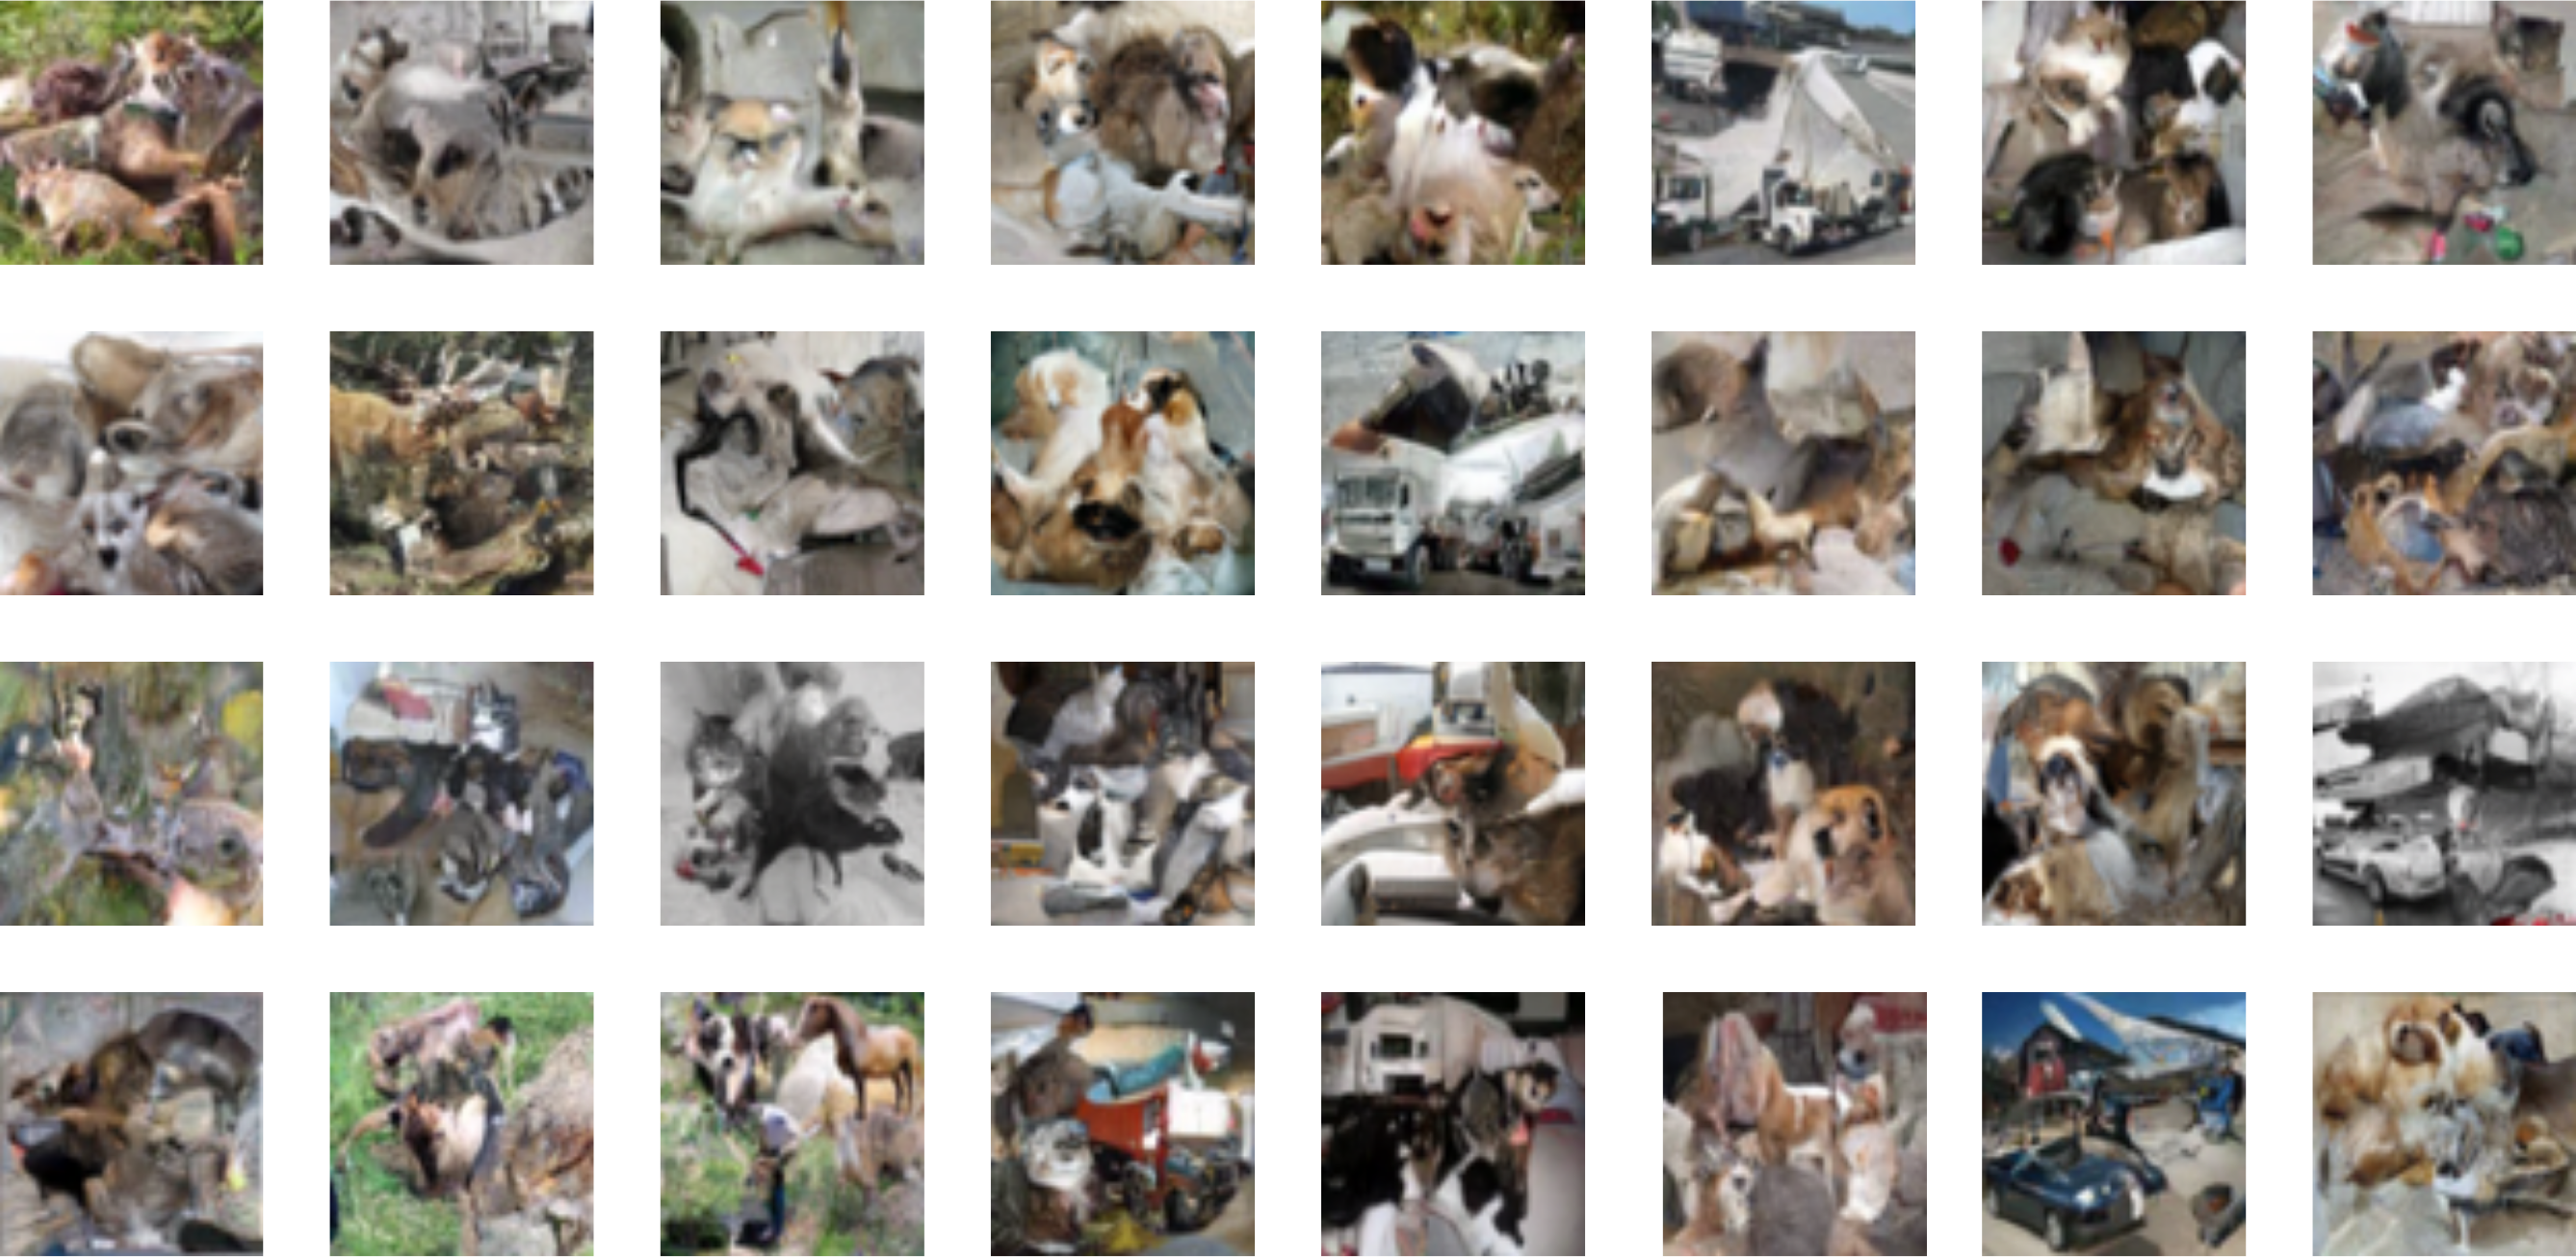
\includegraphics[width=.99\columnwidth]{qbmout.png}
    \caption{\label{fig:qbmresults}QBM-generated image synthesis output from random noise inputs.}
\end{figure}

\subsection{Feature Extraction}
Since QBMs and RBMs both lack convolutional layers, which are especially effective at capturing image features via convolution and image filters, it is expected that they would in turn score poorly for FID scores. This limitation of RBMs and QBMs can be solved by transfer learning. Transfer learning allows a pre-trained model to be detached between two layers and then reconnected to an untrained model. That way, the embeddings, i.e., learned weights of the pre-trained model, can improve the performance of the untrained model~\cite{transfer}. Transfer learning with the convolutional layers from a CNN can be detached and reattached to the visible nodes of the RBM and QBM. However, for this strategy to work as intended with the QBM, a binarization layer, discussed in \hl{Section} \ref{binarize},  would need to interface between the output of the CNN layers and the visible nodes.


\subsection{Trilemma of Generative Learning}
Recall the trilemma consists of the following: ``(i) high-quality sampling, (ii) mode coverage \& sample diversity, and (iii) fast and computationally inexpensive sampling''~\cite{xiao2022DDGAN}.

\subsubsection{High-Quality Sampling}
High-quality sampling is captured by FID and Inception scores. The QBM performed terribly on the Inception score and only moderately well on FID scores. Thus, it would be inaccurate to say the quantum annealer is uniquely producing high-quality samples. We hypothesize the main contributor to this result is the lack of convolutional layers and the image stitching required for training. This will be further discussed in \ref{future}.

\subsubsection{Mode Coverage and Diversity}
Mode coverage and diversity are captured by Inception and KID scores. While the QBM performed poorly on the Inception score, the KID score was promising. From qualitative observations of the generated images, it seems the QBM is managing to produce a diversity of images representative of the training data. The Inception score is certainly poorer than expected due to image stitching causing the Inception classifier to fail at classifying the images into one class.

\subsubsection{Fast Sampling}
The QBM thoroughly and unequivocally fails at fast sampling. The quantum annealer is extremely slow at sampling. This is partially due to hardware constraints, partially due to the high demand for quantum resources, and partially due to computational expensiveness. Regardless, the process of quantum sampling from an annealer is prohibitively slow and expensive. We hope to see this improve over time.

\subsubsection{Conclusions}
\textls[-25]{The QBM currently fails to improve on the Trilemma of Generative Learning (\mbox{\hl{Section}~\ref{trilemmaGL}}}) in any of the three axes in any meaningful way. Despite this lack of improvement, it is important to note that quantum annealers are still in their infancy and have a limited number of qubits, require significant error correcting, are a shared resource, and are not the same as (or have the universality of) a general quantum computer. With hardware improvements, we expect to see further improvements and can revisit the trilemma once significant progress has been made.

\section{Conclusions and Future Work}
\label{future}
In conclusion, our team attempted to determine the efficacy of the D-Wave 2000Q quantum annealer on image synthesis, evaluated by industry-standard metrics compared to classical model counterparts, and determined if QBMs can crack the Trilemma of Generative Learning (\hl{Section} \ref{trilemmaGL}). The quantum annealer, operating under a Quantum Boltzmann Machine (QBM) architecture, was assessed based on several performance metrics, including the Inception score, Fréchet Inception Distance (FID), and Kernel Inception Distance (KID). Its performance was compared against a suite of classical models comprising:
\begin{itemize}
\item Restricted Boltzmann Machine
\item Variational Autoencoder
\item Generative Adversarial Network
\item Denoising Diffusion Probabilistic Model
\end{itemize}


The quantitative results of these experiments can be found in Table~\ref{tab: results}. The results showed that the QBM struggled to generate images with a high Inception score but managed to show promise in FID and KID scores, indicating an ability to generate images with salient features and a similar distribution to that of the training set.


The QBM implemented on the D-Wave 2000Q quantum annealer is not significantly better than the state-of-the-art classical models in the field. While the QBM outperformed a few classical models on FID and KID scores, it is important to note the difficulty of comparing models with different architectures trained on different hyper-parameters. The QBM did show great promise in its ability to represent the underlying distribution of the training data in its generated samples, and we hope to see this improve with more hardware improvements.

\subsection{Image Preprocessing}
A significant challenge in developing the QBM was the lack of qubits. This limitation forced us to split each image into a set of four squares, as described in \hl{Section} \ref{binarize}, leading to the issue of stitching generated images in post. This issue can be somewhat resolved in the future in a few different ways.


Firstly, one could wait until hardware improvements are made to the quantum annealer in the form of an increase in the number of qubits and error-correcting abilities. With these improvements, one should see an increase in image synthesis quality. As more pixels can be embedded directly onto the QPU, the need for stitching will diminish and the QBM will be able to encode a richer embedding with features from the entire image in the correct~locations.


Secondly, a CNN could be introduced and pre-trained via transfer learning. This would limit the input vector size required for the visible nodes on the QBM, thus allowing the CNN to pick up the bulk of the feature extraction. While this would not be a purely ``quantum'' solution, it would allow for the quantum annealer to specialize in embedding and sampling from a distribution of features as opposed to pixel values. This ought to improve performance, as CNNs are the gold standard in image processing for machine learning applications.

\subsection{Quantum Computing}
As quantum annealers improve, our team expects the ability to sample more often and in greater numbers will improve. With a greater number of samples, the QBM can evaluate a richer energy landscape and capture a more sophisticated objective function topology. With faster sampling, additional hyper-tuning could also be performed in a more timely manner, allowing for greater convergence upon a more ideal architecture.%MDPI: Please note that back matters are essential, please carefully check the contri information before resubmitting the file.

\vspace{6pt}

\authorcontributions{\hl{~~~}}%MDPI: For research articles with several authors, a short paragraph specifying their individual contributions must be provided. The following statements should be used ``Conceptualization, X.X. and Y.Y.; methodology, X.X.; software, X.X.; validation, X.X., Y.Y. and Z.Z.; formal analysis, X.X.; investigation, X.X.; resources, X.X.; data curation, X.X.; writing---original draft preparation, X.X.; writing---review and editing, X.X.; visualization, X.X.; supervision, X.X.; project administration, X.X.; funding acquisition, Y.Y. All authors have read and agreed to the published version of the manuscript.'', please turn to the  \href{http://img.mdpi.org/data/contributor-role-instruction.pdf}{CRediT taxonomy} for the term explanation. Authorship must be limited to those who have contributed substantially to the work~reported.

\funding{\hl{~~~}}%MDPI: Please add: ``This research received no external funding'' or ``This research was funded by NAME OF FUNDER grant number XXX.'' and  and ``The APC was funded by XXX''. Check carefully that the details given are accurate and use the standard spelling of funding agency names at \url{https://search.crossref.org/funding}, any errors may affect your future funding.

\institutionalreview{\hl{~~~}}%MDPI: In this section, you should add the Institutional Review Board Statement and approval number, if relevant to your study. You might choose to exclude this statement if the study did not require ethical approval. Please note that the Editorial Office might ask you for further information. Please add “The study was conducted in accordance with the Declaration of Helsinki, and approved by the Institutional Review Board (or Ethics Committee) of NAME OF INSTITUTE (protocol code XXX and date of approval).” for studies involving humans. OR “The animal study protocol was approved by the Institutional Review Board (or Ethics Committee) of NAME OF INSTITUTE (protocol code XXX and date of approval).” for studies involving animals. OR “Ethical review and approval were waived for this study due to REASON (please provide a detailed justification).” OR “Not applicable” for studies not involving humans or animals.

\informedconsent{\hl{~~~}}%MDPI: Any research article describing a study involving humans should contain this statement. Please add ``Informed consent was obtained from all subjects involved in the study.'' OR ``Patient consent was waived due to REASON (please provide a detailed justification).'' OR ``Not applicable'' for studies not involving humans. You might also choose to exclude this statement if the study did not involve humans. Written informed consent for publication must be obtained from participating patients who can be identified (including by the patients themselves). Please state ``Written informed consent has been obtained from the patient(s) to publish this paper'' if applicable. 

\dataavailability{\hl{~~~}}%MDPI: We encourage all authors of articles published in MDPI journals to share their research data. In this section, please provide details regarding where data supporting reported results can be found, including links to publicly archived datasets analyzed or generated during the study. Where no new data were created, or where data is unavailable due to privacy or ethical restrictions, a statement is still required. Suggested Data Availability Statements are available in section ``MDPI Research Data Policies'' at \url{https://www.mdpi.com/ethics}.  

\acknowledgments{\hl{We would} %MDPI: Titles (e.g., Dr., Mr., and Prof.) should NOT be used in the Acknowledgments section. please remove them. 
 like to thank D-Wave for providing access to their quantum computing resources as well as their continued support for Quantum Machine Learning research. This research would not be possible without the deep collaboration with Nurosene Health and their Chief Scientific Officer \hl{Dr.} Joseph Geraci, \hl{Assistant Professor} at Queen’s Molecular Medicine. Lastly, a special thank you to \hl{Prof.} Harry Ruda, Stanley Meek \hl{Chair} in Advanced Nanotechnology, and \hl{Professor} in the Department of Material Science and Engineering at the University of Toronto, for supervising this~research.}%MDPI: Please clarify if the authors have collaborated with a company/business scene without receving any funds from the aforementioned company, that this research was conducted in the absence  of any commercial or financial relationships that could be construed as a  potential conflict of interest. For more information, please see 'Conflicts of Interest' section in: https://www.mdpi.com/journal/technologies/instructions 

\conflictsofinterest{\hl{~~~}}%MDPI: Please clarify if the authors have collaborate with a company/business scene, and declare conflicts of interest or state ``The authors declare no conflicts of interest.'' Authors must identify and declare any personal circumstances or interest that may be perceived as inappropriately influencing the representation or interpretation of reported research results. Any role of the funders in the design of the study; in the collection, analyses or interpretation of data; in the writing of the manuscript; or in the decision to publish the results must be declared in this section. If there is no role, please state ``The funders had no role in the design of the study; in the collection, analyses, or interpretation of data; in the writing of the manuscript; or in the decision to publish the results''. 

 
\begin{adjustwidth}{-\extralength}{0cm} 
\reftitle{References}
 \begin{thebibliography}{999}

\bibitem[Ho et~al.(2020)Ho, Jain, and Abbeel]{ho2020denoising}
Ho, J.; Jain, A.; Abbeel, P.
\newblock Denoising Diffusion Probabilistic Models.
\newblock In \emph{Advances in Neural Information Processing
  Systems}; Larochelle, H., Ranzato, M., Hadsell, R., Balcan, M., Lin, H., Eds.; Curran Associates, Inc.: \hl{Red Hook, NY, USA}%MDPI: We formated as book and added the location of the publisher. Please confirm.
, 2020; Volume~33, pp. 6840--6851.

\bibitem[Dhariwal and Nichol(2021)]{dhariwal2021diffusion}
Dhariwal, P.; Nichol, A.
\newblock Diffusion Models Beat GANs on Image Synthesis. \emph{arXiv} \textbf{2021}, \hl{arXiv:2105.05233}%MDPI: We changed link. Please confirm this revision.
.

\bibitem[Jain et~al.(2020)Jain, Ziauddin, Leonchyk, Yenkanchi, and
  Geraci]{Jain2020}
Jain, S.; Ziauddin, J.; Leonchyk, P.; Yenkanchi, S.; Geraci, J.
\newblock Quantum and classical machine learning for the classification of
  non-small-cell lung cancer patients.
\newblock {\em {SN} Appl. Sci.} {\bf 2020}, {\em 2}, \hl{1088}%MDPI: Newly added information. Please confirm. same below.
.
\newblock {\url{https://doi.org/10.1007/s42452-020-2847-4}}.

\bibitem[Thulasidasan()]{Thulasidasan2016}
Thulasidasan, S.
\newblock \emph{Generative Modeling for Machine Learning on the D-Wave}; \hl{Technical Report;  Los Alamos National Lab. (LANL): Los Alamos, NM, USA, 2016.} {\url{https://doi.org/10.2172/1332219}}.

\bibitem[Amin et~al.(2018)Amin, Andriyash, Rolfe, Kulchytskyy, and
  Melko]{Amin_2018}
Amin, M.H.; Andriyash, E.; Rolfe, J.; Kulchytskyy, B.; Melko, R.
\newblock Quantum Boltzmann Machine.
\newblock {\em Phys. Rev. X} {\bf 2018}, {\em 8},~021050.
\newblock {\url{https://doi.org/10.1103/PhysRevX.8.021050}}.

\bibitem[Xiao et~al.(2021)Xiao, Kreis, and Vahdat]{xiao2022DDGAN}
\textls[-25]{Xiao, Z.; Kreis, K.; Vahdat, A. Tackling the Generative Learning Trilemma with Denoising Diffusion GANs. {\em arXiv} {\bf 2021}, \hl{arXiv:2112.07804}.}

\bibitem[Smolensky(1986)]{Smolensky1986InformationPI}
Smolensky, P. Information processing in dynamical systems: Foundations of harmony theory. In {\em Parallel Distributed Processing: Explorations in the Microstructure of Cognition: Foundations}; MIT Press:  \hl{Cambridge, MA, USA,} %We added the location of publisher. Please confirm
 1986; Volume 1.

\bibitem[Freund and Haussler(1991)]{NIPS1991_33e8075e}
Freund, Y.; Haussler, D.
\newblock Unsupervised learning of distributions on binary vectors using two
  layer networks.
\newblock In \emph{Advances in Neural Information Processing
  Systems}; Moody, J., Hanson, S., Lippmann, R., Eds.; Morgan-Kaufmann: \hl{Burlington, MA, USA}, 1991; Volume~4.

\bibitem[Hopfield(1982)]{hopfield}
Hopfield, J.J.
\newblock Neural networks and physical systems with emergent collective
  computational abilities.
\newblock {\em Proc. Natl. Acad. Sci. USA} {\bf 1982},
  {\em 79},~2554--2558.  {\url{https://doi.org/10.1073/pnas.79.8.2554}}.

\bibitem[Hinton(2012)]{Hinton2012}
Hinton, G.E.
\newblock A Practical Guide to Training Restricted Boltzmann Machines. In {\em   Lecture Notes in Computer Science}; Springer:  \hl{Berlin/Heidelberg, Germany,} %We added the location of publisher. Please confirm
  2012; pp. 599--619. {\url{https://doi.org/10.1007/978-3-642-35289-8_32}}.

\bibitem[Carreira-Perpi{\~n}{\'a}n and Hinton(2005)]{CarreiraPerpin2005OnCD}
Carreira-Perpi{\~n}{\'a}n, M.{\'A}.; Hinton, G.E. On Contrastive Divergence Learning. In Proceedings of the AISTATS, \hl{Bridgetown, Barbados, 6--8 January 2005}. %MDPI: We added the location and date of the conference. Please confirm.


\bibitem[Kingma and Welling(2014)]{kingma2014autoencoding}
Kingma, D.P.; Welling, M. Auto-Encoding Variational Bayes.  \emph{arXiv} \textbf{2014},  \hl{arXiv:1312.6114}.

\bibitem[Rocca(2021)]{rocca_2021}
Rocca, J. Understanding Variational Autoencoders (VAES). 2021.  Available online: \url{https://towardsdatascience.com/understanding-variational-autoencoders-vaes-f70510919f73} (\hl{accessed on}%MDPI: Please add the access date (format: Date Month Year), e.g., accessed on 1 January 2020. same below.
). 

\bibitem[Goodfellow et~al.(2014)Goodfellow, Pouget-Abadie, Mirza, Xu,
  Warde-Farley, Ozair, Courville, and Bengio]{goodfellow2014generative}
Goodfellow, I.J.; Pouget-Abadie, J.; Mirza, M.; Xu, B.; Warde-Farley, D.;
  Ozair, S.; Courville, A.; Bengio, Y.
\newblock Generative Adversarial Networks. \emph{arXiv} \textbf{2014},  \hl{ arXiv:1406.2661}.  

\bibitem[pat()]{pathmind}
A Beginner's Guide to Generative Adversarial Networks (Gans). Available online: \url{https://wiki.pathmind.com/generative-adversarial-network-gan} (\hl{accessed on}).

\bibitem[Arjovsky and Bottou(2017)]{google}
Arjovsky, M.; Bottou, L. Towards Principled Methods for Training Generative Adversarial Networks. \emph{arXiv} \textbf{2017},  \hl{arXiv:1701.04862}.
 

\bibitem[Hinton(2002)]{trainingrbms}
Hinton, G.E.
\newblock Training Products of Experts by Minimizing Contrastive Divergence.
\newblock {\em Neural Comput.} {\bf 2002}, {\em 14},~1771--1800.
\newblock {\url{https://doi.org/10.1162/089976602760128018}}.

\bibitem[dwa()]{dwavedocs}
{W}hat is {Q}uantum {A}nnealing? {D}-{W}ave {S}ystem {D}ocumentation.
 Available online: \url{https://docs.dwavesys.com/docs/latest/c_gs_2.html} (\hl{accessed on}). 

\bibitem[Lu et~al.(2023)Lu, Liu, Song, Wen, and Wang]{monte}
Lu, B.; Liu, L.; Song, J.Y.; Wen, K.; Wang, C.
\newblock Recent progress on coherent computation based on quantum squeezing. {\em {AAPPS} Bull.} {\bf 2023}, {\em 33}, \hl{7}. {\url{https://doi.org/10.1007/s43673-023-00077-4}}.

\bibitem[Wittek and Gogolin(2017)]{qpugibbs}
Wittek, P.; Gogolin, C.
\newblock Quantum Enhanced Inference in Markov Logic Networks.
\newblock {\em Sci. Rep.} {\bf 2017}, {\em 7},~45672. {\url{https://doi.org/10.1038/srep45672}}.

\bibitem[Li and Deng(2022)]{classifiers}
Li, W.; Deng, D.L.
\newblock Recent advances for quantum classifiers.
\newblock {\em Sci. China Phys. Mech. Astron.} {\bf 2022}, {\em
  65},~220301.  {\url{https://doi.org/10.1007/s11433-021-1793-6}}.

\bibitem[Wei et~al.(2022)Wei, Chen, Zhou, and Long]{quantumCNN}
Wei, S.; Chen, Y.; Zhou, Z.; Long, G.
\newblock A quantum convolutional neural network on NISQ devices.
\newblock {\em AAPPS Bull.} {\bf 2022}, {\em 32}, \hl{2}.
\newblock {\url{https://doi.org/10.1007/s43673-021-00030-3}}.

\bibitem[Sleeman et~al.(2020)Sleeman, Dorband, and Halem]{qmlimggen}
Sleeman, J.; Dorband, J.E.; Halem, M.
\newblock A hybrid quantum enabled RBM advantage: Convolutional autoencoders
  for quantum image compression and generative learning. \emph{arXiv} \textbf{2020},  \hl{arXiv:2001.11946}.

\bibitem[Krizhevsky et~al.()Krizhevsky, Nair, and Hinton]{CIFAR}
Krizhevsky, A.; Nair, V.; Hinton, G.
\newblock \hl{CIFAR-10 (Canadian Institute for Advanced Research).}%MDPI: Please provide more information about the article type, such as book (please provide the name and location of the publisher); online resource (please provide the URL of the website and the date it was accessed (Date Month Year)); or journal article (please provide the name of the journal, the year and volume in which it was published, and the page number). Please refer to https://www.mdpi.com/authors/references for full reference formatting guides.


\bibitem[Krizhevsky(2009)]{Krizhevsky09learningmultiple}
Krizhevsky, A.
\newblock Learning Multiple Layers of Features from Tiny Images.
\newblock  2009. Available online: \url{https://www.cs.toronto.edu/~kriz/learning-features-2009-TR.pdf} (\hl{accessed on}).

\bibitem[Peter~Eckersley(2017)]{ai_progress_measurement}
\hl{Peter~Eckersley, Y.N.e.a.} %MDPI: Please provide the correct author names.
\newblock \hl{EFF AI Progress Measurement Project. 2017}%MDPI: Please provide more information about the article type, such as book (please provide the name and location of the publisher); online resource (please provide the URL of the website and the date it was accessed (Date Month Year)); or journal article (please provide the name of the journal, the year and volume in which it was published, and the page number). Please refer to https://www.mdpi.com/authors/references for full reference formatting guides.
.

\bibitem[Mack(2019)]{mack_2019}
Mack, D. A Simple Explanation of the Inception Score. 2019. Available online: \url{https://medium.com/octavian-ai/a-simple-explanation-of-the-inception-score-372dff6a8c7a} (\hl{accessed on}).

\bibitem[Szegedy et~al.(2015)Szegedy, Vanhoucke, Ioffe, Shlens, and
  Wojna]{inception_model}
Szegedy, C.; Vanhoucke, V.; Ioffe, S.; Shlens, J.; Wojna, Z.
\newblock Rethinking the Inception Architecture for Computer Vision.   \emph{arXiv} \textbf{2015},  \hl{arXiv:1512.00567}. 

\bibitem[Salimans et~al.(2016)Salimans, Goodfellow, Zaremba, Cheung, Radford,
  and Chen]{isscore}
Salimans, T.; Goodfellow, I.; Zaremba, W.; Cheung, V.; Radford, A.; Chen, X.
\newblock Improved Techniques for Training GANs. \emph{arXiv} \textbf{2016},  \hl{arXiv:1606.03498}. 

\bibitem[Heusel et~al.(2017{\natexlab{a}})Heusel, Ramsauer, Unterthiner,
  Nessler, and Hochreiter]{NIPS2017_8a1d6947}
Heusel, M.; Ramsauer, H.; Unterthiner, T.; Nessler, B.; Hochreiter, S.
\newblock GANs Trained by a Two Time-Scale Update Rule Converge to a Local Nash
  Equilibrium. In \emph{Advances in Neural Information Processing
  Systems}; Guyon, I., Luxburg, U.V., Bengio, S., Wallach, H., Fergus, R.,
  Vishwanathan, S., Garnett, R., Eds.; Curran Associates, Inc.: \hl{Red Hook, NY, USA,} 2017; Volume~30.%MDPI: Please carefully check if this and next reference are duplicated, please consider changing the reference and reorganize the citation order throughout the manuscript in case these two references were the same paper

\bibitem[Heusel et~al.(2017{\natexlab{b}})Heusel, Ramsauer, Unterthiner,
  Nessler, and Hochreiter]{fid_gan}
Heusel, M.; Ramsauer, H.; Unterthiner, T.; Nessler, B.; Hochreiter, S.
\newblock GANs Trained by a Two Time-Scale Update Rule Converge to a Local Nash
  Equilibrium. \emph{arXiv} \textbf{2017},  \hl{arXiv:1706.08500}.  
 {\url{https://doi.org/10.48550/ARXIV.1706.08500}}.

\bibitem[Bińkowski et~al.(2018)Bińkowski, Sutherland, Arbel, and
  Gretton]{MMD_KID}
Bińkowski, M.; Sutherland, D.J.; Arbel, M.; Gretton, A.
\newblock Demystifying MMD GANs.  \emph{arXiv} \textbf{2018},  \hl{arXiv:1801.01401}.   {\url{https://doi.org/10.48550/ARXIV.1801.01401}}.

\bibitem[goo()]{googlecloud}
Cloud Tensor Processing Units (TPUS)|Google Cloud. Available online: \url{https://cloud.google.com/tpu/docs/tpus} (\hl{accessed~on}). 

\bibitem[Dhillon et~al.(2009)Dhillon, Foster, and Ungar]{transfer}
Dhillon, P.S.; Foster, D.; Ungar, L.  Transfer Learning Using Feature Selection.  \emph{arXiv} \textbf{2009},  \hl{arXiv:0905.4022}. {\url{https://doi.org/10.48550/ARXIV.0905.4022}}.

\end{thebibliography}

\PublishersNote{}
\end{adjustwidth}
\end{document} 